\documentclass[tikz,border=5pt]{standalone}
\begin{document}
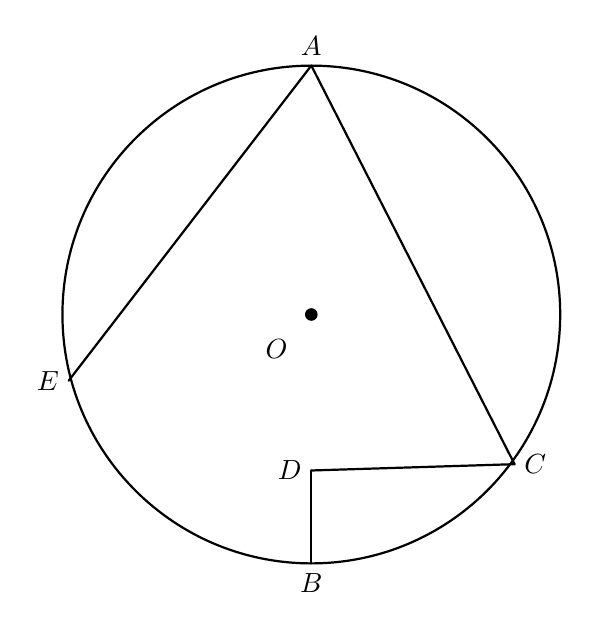
\begin{tikzpicture}[scale=0.02, line cap=round, line join=round]
  % 坐标（以 O 为原点）
  \coordinate (O) at (0,0);
  \coordinate (A) at (0,158);
  \coordinate (B) at (0,-158);
  \coordinate (E) at (-154,-42);
  \coordinate (C) at (129,-95);
  \coordinate (D) at (0,-99);

  % 圆
  \draw[thick] (O) circle (158);

  % 线段（已删除线段 AD 的笔画）
  \draw[thick] (A) -- (E);
  \draw[thick] (A) -- (C);
  \draw[thick] (D) -- (C);
  \draw[thick] (D) -- (B);

  % 圆心
  \fill (O) circle (4);

  % 标签
  \node[above] at (A) {$A$};
  \node[below] at (B) {$B$};
  \node at (-22,-22) {$O$};
  \node[left] at (D) {$D$};
  \node[right] at (C) {$C$};
  \node[left] at (E) {$E$};
\end{tikzpicture}
\end{document}
